\documentclass[twoside]{book}

% Packages required by doxygen
\usepackage{fixltx2e}
\usepackage{calc}
\usepackage{doxygen}
\usepackage[export]{adjustbox} % also loads graphicx
\usepackage{graphicx}
\usepackage[utf8]{inputenc}
\usepackage{makeidx}
\usepackage{multicol}
\usepackage{multirow}
\PassOptionsToPackage{warn}{textcomp}
\usepackage{textcomp}
\usepackage[nointegrals]{wasysym}
\usepackage[table]{xcolor}

% Font selection
\usepackage[T1]{fontenc}
\usepackage[scaled=.90]{helvet}
\usepackage{courier}
\usepackage{amssymb}
\usepackage{sectsty}
\renewcommand{\familydefault}{\sfdefault}
\allsectionsfont{%
  \fontseries{bc}\selectfont%
  \color{darkgray}%
}
\renewcommand{\DoxyLabelFont}{%
  \fontseries{bc}\selectfont%
  \color{darkgray}%
}
\newcommand{\+}{\discretionary{\mbox{\scriptsize$\hookleftarrow$}}{}{}}

% Page & text layout
\usepackage{geometry}
\geometry{%
  a4paper,%
  top=2.5cm,%
  bottom=2.5cm,%
  left=2.5cm,%
  right=2.5cm%
}
\tolerance=750
\hfuzz=15pt
\hbadness=750
\setlength{\emergencystretch}{15pt}
\setlength{\parindent}{0cm}
\setlength{\parskip}{3ex plus 2ex minus 2ex}
\makeatletter
\renewcommand{\paragraph}{%
  \@startsection{paragraph}{4}{0ex}{-1.0ex}{1.0ex}{%
    \normalfont\normalsize\bfseries\SS@parafont%
  }%
}
\renewcommand{\subparagraph}{%
  \@startsection{subparagraph}{5}{0ex}{-1.0ex}{1.0ex}{%
    \normalfont\normalsize\bfseries\SS@subparafont%
  }%
}
\makeatother

% Headers & footers
\usepackage{fancyhdr}
\pagestyle{fancyplain}
\fancyhead[LE]{\fancyplain{}{\bfseries\thepage}}
\fancyhead[CE]{\fancyplain{}{}}
\fancyhead[RE]{\fancyplain{}{\bfseries\leftmark}}
\fancyhead[LO]{\fancyplain{}{\bfseries\rightmark}}
\fancyhead[CO]{\fancyplain{}{}}
\fancyhead[RO]{\fancyplain{}{\bfseries\thepage}}
\fancyfoot[LE]{\fancyplain{}{}}
\fancyfoot[CE]{\fancyplain{}{}}
\fancyfoot[RE]{\fancyplain{}{\bfseries\scriptsize Generated by Doxygen }}
\fancyfoot[LO]{\fancyplain{}{\bfseries\scriptsize Generated by Doxygen }}
\fancyfoot[CO]{\fancyplain{}{}}
\fancyfoot[RO]{\fancyplain{}{}}
\renewcommand{\footrulewidth}{0.4pt}
\renewcommand{\chaptermark}[1]{%
  \markboth{#1}{}%
}
\renewcommand{\sectionmark}[1]{%
  \markright{\thesection\ #1}%
}

% Indices & bibliography
\usepackage{natbib}
\usepackage[titles]{tocloft}
\setcounter{tocdepth}{3}
\setcounter{secnumdepth}{5}
\makeindex

% Hyperlinks (required, but should be loaded last)
\usepackage{ifpdf}
\ifpdf
  \usepackage[pdftex,pagebackref=true]{hyperref}
\else
  \usepackage[ps2pdf,pagebackref=true]{hyperref}
\fi
\hypersetup{%
  colorlinks=true,%
  linkcolor=blue,%
  citecolor=blue,%
  unicode%
}

% Custom commands
\newcommand{\clearemptydoublepage}{%
  \newpage{\pagestyle{empty}\cleardoublepage}%
}

\usepackage{caption}
\captionsetup{labelsep=space,justification=centering,font={bf},singlelinecheck=off,skip=4pt,position=top}

%===== C O N T E N T S =====

\begin{document}

% Titlepage & ToC
\hypersetup{pageanchor=false,
             bookmarksnumbered=true,
             pdfencoding=unicode
            }
\pagenumbering{alph}
\begin{titlepage}
\vspace*{7cm}
\begin{center}%
{\Large Package for manipulating messages on topics }\\
\vspace*{1cm}
{\large Generated by Doxygen 1.8.13}\\
\end{center}
\end{titlepage}
\clearemptydoublepage
\pagenumbering{roman}
\tableofcontents
\clearemptydoublepage
\pagenumbering{arabic}
\hypersetup{pageanchor=true}

%--- Begin generated contents ---
\chapter{Hierarchical Index}
\section{Class Hierarchy}
This inheritance list is sorted roughly, but not completely, alphabetically\+:\begin{DoxyCompactList}
\item \contentsline{section}{Message\+Filter\+Base$<$ T $>$}{\pageref{classMessageFilterBase}}{}
\begin{DoxyCompactList}
\item \contentsline{section}{Message\+Mean\+Filter$<$ T $>$}{\pageref{classMessageMeanFilter}}{}
\end{DoxyCompactList}
\end{DoxyCompactList}

\chapter{Class Index}
\section{Class List}
Here are the classes, structs, unions and interfaces with brief descriptions\+:\begin{DoxyCompactList}
\item\contentsline{section}{\hyperlink{classMessageFilterBase}{Message\+Filter\+Base$<$ T $>$} \\*Base class for topic filters (convulutional filters) }{\pageref{classMessageFilterBase}}{}
\item\contentsline{section}{\hyperlink{classMessageMeanFilter}{Message\+Mean\+Filter$<$ T $>$} \\*Class that implements a mean filter for a given Topic type }{\pageref{classMessageMeanFilter}}{}
\end{DoxyCompactList}

\chapter{Class Documentation}
\hypertarget{classMessageFilterBase}{}\section{Message\+Filter\+Base$<$ T $>$ Class Template Reference}
\label{classMessageFilterBase}\index{Message\+Filter\+Base$<$ T $>$@{Message\+Filter\+Base$<$ T $>$}}


Base class for topic filters (convulutional filters)  




{\ttfamily \#include $<$msg\+\_\+filter\+\_\+base.\+hpp$>$}



<<<<<<< HEAD
Inheritance diagram for Message\+Filter\+Base$<$ T $>$\+:\nopagebreak
=======
Inheritance diagram for Message\+Filter\+Base$<$ T $>$\+:
\nopagebreak
>>>>>>> 3a0e2fbc2a072cb3e232d095681eda1e3dcdebcb
\begin{figure}[H]
\begin{center}
\leavevmode
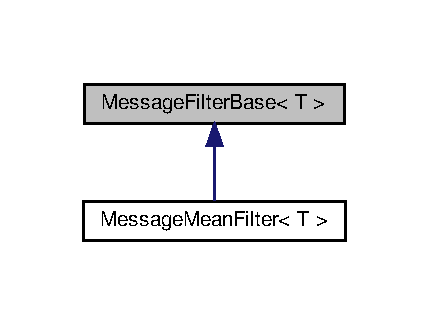
\includegraphics[width=206pt]{d3/d58/classMessageFilterBase__inherit__graph}
\end{center}
\end{figure}
\subsection*{Public Member Functions}
\begin{DoxyCompactItemize}
\item 
\hyperlink{classMessageFilterBase_aeb8e41a157fef0bcf63bd8061eea4b4a}{Message\+Filter\+Base} (ros\+::\+Node\+Handle \&nh)
\begin{DoxyCompactList}\small\item\em Construct a new Message Filter Base object. \end{DoxyCompactList}\end{DoxyCompactItemize}
\subsection*{Protected Member Functions}
\begin{DoxyCompactItemize}
\item 
virtual T \hyperlink{classMessageFilterBase_a9ddc835d7366cacf63ba4a4e42839f6b}{filter} ()=0
\begin{DoxyCompactList}\small\item\em Procedure the filter algorithm is implemented in. \end{DoxyCompactList}\end{DoxyCompactItemize}
\subsection*{Protected Attributes}
\begin{DoxyCompactItemize}
\item 
\mbox{\Hypertarget{classMessageFilterBase_a0b7db0e443e75ce02ef154f233adc97d}\label{classMessageFilterBase_a0b7db0e443e75ce02ef154f233adc97d}} 
std\+::unique\+\_\+ptr$<$ boost\+::circular\+\_\+buffer$<$ T $>$ $>$ {\bfseries buffer\+\_\+}
\end{DoxyCompactItemize}


\subsection{Detailed Description}
\subsubsection*{template$<$class T$>$\newline
class Message\+Filter\+Base$<$ T $>$}

\tabulinesep=1mm
\begin{longtabu} spread 0pt [c]{*{2}{|X[-1]}|}
\hline
\rowcolor{\tableheadbgcolor}\textbf{ Subscribed Topic}&\textbf{ Description  }\\\cline{1-2}
\endfirsthead
\hline
\endfoot
\hline
\rowcolor{\tableheadbgcolor}\textbf{ Subscribed Topic}&\textbf{ Description  }\\\cline{1-2}
\endhead
input&The topic the value to be filtered is published at \\\cline{1-2}
output&The topic the filtered value is published at \\\cline{1-2}
\end{longtabu}
<<<<<<< HEAD


=======
\tabulinesep=1mm
\begin{longtabu} spread 0pt [c]{*{2}{|X[-1]}|}
\hline
\rowcolor{\tableheadbgcolor}\textbf{ Ros-\/\+Parameter}&\textbf{ Desciption  }\\\cline{1-2}
\endfirsthead
\hline
\endfoot
\hline
\rowcolor{\tableheadbgcolor}\textbf{ Ros-\/\+Parameter}&\textbf{ Desciption  }\\\cline{1-2}
\endhead
$\sim$sample\+\_\+number$<$td$>$Number of samples the mean is calculated from \\\cline{1-2}
\end{longtabu}
>>>>>>> 3a0e2fbc2a072cb3e232d095681eda1e3dcdebcb

\begin{DoxyTemplParams}{Template Parameters}
{\em T} & Tpye of the Message to be filtered. Operators for the derived filteres must be implemented. \\
\hline
\end{DoxyTemplParams}


\subsection{Constructor \& Destructor Documentation}
\mbox{\Hypertarget{classMessageFilterBase_aeb8e41a157fef0bcf63bd8061eea4b4a}\label{classMessageFilterBase_aeb8e41a157fef0bcf63bd8061eea4b4a}} 
\index{Message\+Filter\+Base@{Message\+Filter\+Base}!Message\+Filter\+Base@{Message\+Filter\+Base}}
\index{Message\+Filter\+Base@{Message\+Filter\+Base}!Message\+Filter\+Base@{Message\+Filter\+Base}}
\subsubsection{\texorpdfstring{Message\+Filter\+Base()}{MessageFilterBase()}}
{\footnotesize\ttfamily template$<$class T $>$ \\
\hyperlink{classMessageFilterBase}{Message\+Filter\+Base}$<$ T $>$\+::\hyperlink{classMessageFilterBase}{Message\+Filter\+Base} (\begin{DoxyParamCaption}\item[{ros\+::\+Node\+Handle \&}]{nh }\end{DoxyParamCaption})}


\begin{DoxyParams}{Parameters}
{\em nh} & Nodehandle for handling ros namespaces \\
\hline
\end{DoxyParams}


\subsection{Member Function Documentation}
\mbox{\Hypertarget{classMessageFilterBase_a9ddc835d7366cacf63ba4a4e42839f6b}\label{classMessageFilterBase_a9ddc835d7366cacf63ba4a4e42839f6b}} 
\index{Message\+Filter\+Base@{Message\+Filter\+Base}!filter@{filter}}
\index{filter@{filter}!Message\+Filter\+Base@{Message\+Filter\+Base}}
\subsubsection{\texorpdfstring{filter()}{filter()}}
{\footnotesize\ttfamily template$<$class T $>$ \\
virtual T \hyperlink{classMessageFilterBase}{Message\+Filter\+Base}$<$ T $>$\+::filter (\begin{DoxyParamCaption}{ }\end{DoxyParamCaption})\hspace{0.3cm}{\ttfamily [protected]}, {\ttfamily [pure virtual]}}

Uses values from the buffer\+\_\+ and filters them.

\begin{DoxyReturn}{Returns}
T Filtered value. 
\end{DoxyReturn}


The documentation for this class was generated from the following files\+:\begin{DoxyCompactItemize}
\item 
include/manipulate\+\_\+topics/msg\+\_\+filter\+\_\+base.\+hpp\item 
src/msg\+\_\+filter\+\_\+base.\+cpp\end{DoxyCompactItemize}

\hypertarget{classMessageMeanFilter}{}\section{Message\+Mean\+Filter$<$ T $>$ Class Template Reference}
\label{classMessageMeanFilter}\index{Message\+Mean\+Filter$<$ T $>$@{Message\+Mean\+Filter$<$ T $>$}}


Class that implements a mean filter for a given Topic type.  




{\ttfamily \#include $<$msg\+\_\+mean\+\_\+filter.\+hpp$>$}



Inheritance diagram for Message\+Mean\+Filter$<$ T $>$\+:
\nopagebreak
\begin{figure}[H]
\begin{center}
\leavevmode
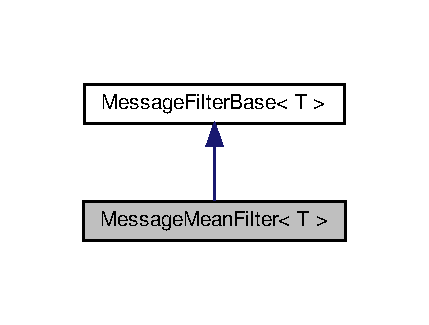
\includegraphics[width=206pt]{dd/d60/classMessageMeanFilter__inherit__graph}
\end{center}
\end{figure}


Collaboration diagram for Message\+Mean\+Filter$<$ T $>$\+:
\nopagebreak
\begin{figure}[H]
\begin{center}
\leavevmode
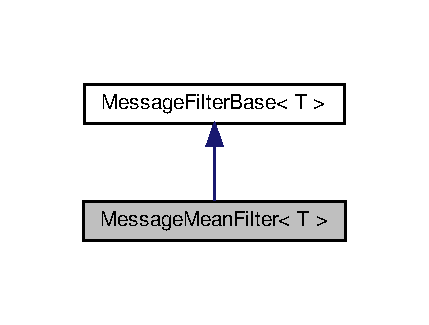
\includegraphics[width=206pt]{d2/db9/classMessageMeanFilter__coll__graph}
\end{center}
\end{figure}
\subsection*{Public Types}
\begin{DoxyCompactItemize}
\item 
\mbox{\Hypertarget{classMessageMeanFilter_aabbf6eb4a2e2251228ece38f88609d29}\label{classMessageMeanFilter_aabbf6eb4a2e2251228ece38f88609d29}} 
typedef boost\+::accumulators\+::accumulator\+\_\+set$<$ T, boost\+::accumulators\+::stats$<$ boost\+::accumulators\+::tag\+::mean $>$ $>$ {\bfseries accumulator}
\end{DoxyCompactItemize}
\subsection*{Public Member Functions}
\begin{DoxyCompactItemize}
\item 
\mbox{\Hypertarget{classMessageMeanFilter_a613460b271336914553f2beb05f4da9b}\label{classMessageMeanFilter_a613460b271336914553f2beb05f4da9b}} 
{\bfseries Message\+Mean\+Filter} (ros\+::\+Node\+Handle \&nh)
\end{DoxyCompactItemize}
\subsection*{Additional Inherited Members}


\subsection{Detailed Description}
\subsubsection*{template$<$class T$>$\newline
class Message\+Mean\+Filter$<$ T $>$}


\begin{DoxyTemplParams}{Template Parameters}
{\em T} & Type of the topic to be filtered. Operators + and / must be implemented within the msg\+\_\+operators namespace. \\
\hline
\end{DoxyTemplParams}


The documentation for this class was generated from the following files\+:\begin{DoxyCompactItemize}
\item 
include/manipulate\+\_\+topics/msg\+\_\+mean\+\_\+filter.\+hpp\item 
src/msg\+\_\+mean\+\_\+filter.\+cpp\end{DoxyCompactItemize}

%--- End generated contents ---

% Index
\backmatter
\newpage
\phantomsection
\clearemptydoublepage
\addcontentsline{toc}{chapter}{Index}
\printindex

\end{document}
